\documentclass[]{article}
\usepackage{amsmath}
\usepackage{amsthm}
\usepackage{amssymb}
\usepackage{graphicx}

\title{Practical Lab Numerical Computing Computational Finance \\Bachelor-Worksheet 1}
\author{Lukas Troska, Ilja Kalmykov}
\date{}
\setlength{\parindent}{0pt}

\begin{document}

\maketitle 
\section*{Task 1} The program outputs uniformly distributed random
numbers between 0 and 1 in two ways, once by the built-in c++-function rand, and
once using gsl.

Removing (double) in the marked line leads to the result being an int (and thus
either 0 or 1, mostly 0), since dividing an int by an int in c++ gives an int,
so we have to cast one of the variables to double to force a floating point
number as the result.

There is a direct function for simulating normally distributed random variables:
double gsl\_ran\_gaussian(const gsl\_rng* r, double sigma), which returns a
gaussian random variable with mean 0 and variance sigma.

\section*{Task 2}
For code see WS1T32.cpp.

\section*{Task 3} The matlab script plots the data against a unit gaussian
probability density function. It first creates a histogram of the data, where it
sorts the numbers into 100 different bins, and then counts the amount of numbers
in each bin. Then it scales the amount of these numbers to show the relative
amount in each bin and plots it against the unit gaussian probability density
function.

The problem in fig. 1 is that $[-2,2]$ is not a good enough bound since the
integral comes out to $\approx 0.95$, thus we get a lot more variables where
$y\le p(x')$ (since it is more likely for an element of $[-2,2]$ then say
$[-3,3]$ to fullfill that), and thus the simulated density has a higher mean
than it should be.

\section*{Task 4} We get a normally distributed random variable if we apply the
inverse of the cdf of the gaussian to the uniform random variable.

\begin{proof}
Let U be a standard uniform random variable, F like in the problem. Then
$P\left[X\le x\right]=P\left[F^{-1}(U) \le x\right]=P\left[U \le
F(x)\right]=F(x)$ (2nd equality holds because F is right-continuous, 3rd
equality holds because U is uniform on [0,1])
\end{proof}

Intuitively this is clear, too: We uniformly choose a number between 0 and 1 and
interpret that as a proportion of the area under the gaussian curve. Then we
return the number that has this proportion of the area on the left of it. Thus,
we are unlikely to choose a number in the tails, since there is little area in
the tails, so we would have to get pick a number very close to 0, whereas for
the other areas we have more "room" so we are more likely to get these.

\section*{Task 5} Firstly, the cdf of the gaussian is pointsymmetric w.r.t. the
y-intercept, thus we can handle the case $x<0$ by $1-NormalCDF(-x)$. If $x>6$,
we know that a normally distributed random variable is guaranteed to be smaller,
thus we return 1. For the other 2 cases: for $0\le x\le 1.87$, its easy to see
that the term given in the return is very close to the cdf of the gaussian since
it behaves almost like a polynomial in that area. For the last case the values
of the cdf are very close to 1, and again like above the given term gives us a
good approximation of the difference of the cdf's value to 1 in that area.

\section*{Task 6} For code see WS1T36.cpp.
\begin{figure}[!ht]
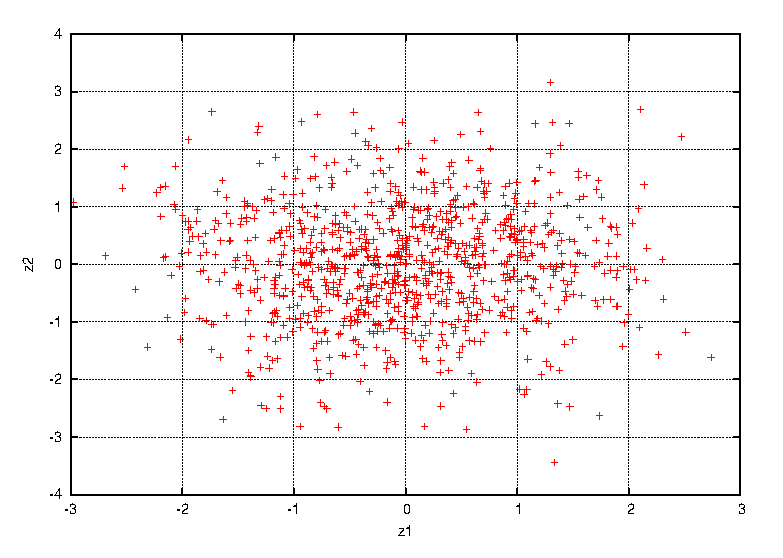
\includegraphics{task6}
\caption{Box-Muller method, 1000 samples}
\label{fig:Task6}
\end{figure}
\clearpage

\section*{Task 7} Let $g_1(u_1,u_2)=\sqrt{-2\log(u_1)}\cos(2\pi
u_2),g_2(u_1,u_2)=\sqrt{-2\log(u_1)}\sin(2\pi u_2)$ be the transformation
(denoted as $z_1, z_2$ in the problem). Solving for $u_1,u_2$ gives us $u_1 =
\exp({-(z_1 ^2+ z_2 ^2)/2}),u_2 = (1/2\pi)\tan^{-1} (z_2/z_1)$. The joint
distribution of $z_1, z_2$ is described by $ f(z_1 ,z_2) = f_{u_1,
u_2}(g_1^{-1}(z_1,z_2),g_2^{-1}(z_1,z_2)) * | J(g) |$ where $J(g)$ is the
Jacobion matrix of the transformation. Plugging both in we get
$f(z_1,z_2)=(\exp(-({z_1}^2+{z_2}^2)/2))/(2\pi)=-(\exp(({z_1}^2/2))/\sqrt{2\pi}*\exp(({z_1}^2/2))/\sqrt{2\pi}$.
We see that $z_1,z_2$ are independent and standard normally distributed.

\section*{Task 8} The advantage of this algorithm is that it is more precise, we
don't have a lot of floating point errors. The variable alpha in the algorithm
is the estimated mean. It is the same as the naive computation because: 
\begin{eqnarray}
    \hat{\mu}_n &= &\frac{1}{N}\sum_{i=1}^n x_i\nonumber\\
    &=&\frac{1}{N}\sum_{i=1}^{n-1}x_i+\frac{1}{N}x_n\nonumber\\
    &=&\frac{\hat{\mu}_{n-1}\left(N-1\right)+x_n}{N}\label{eqn:meanAlg}
\end{eqnarray}

and
\begin{eqnarray}
    \hat{\sigma}^{2}_n\left(N-1\right) &= &\sum_{i=1}^n
    \left(x_i-\mu\right)^2\nonumber\\
    &=&\sum_{i=1}^{n-1}\left(x_i-\mu\right)^2
    +\left(x_n-\mu\right)^2\nonumber\\
    &=&\left(N-2\right)\hat{\sigma}^{2}_{n-1} +
    \left(x_n-\mu\right)^2\label{eqn:varAlg}
\end{eqnarray}

Let $x_n$ be the n-th value, $\hat{\mu}_n$ and $\hat{\sigma}_n$ be the n-th
estimated mean value and variance.  For the variables in the
algorithm we have:
\[\gamma=x_n-\hat{\mu}_{n-1},\quad \alpha=\hat{\mu}_{n-1},\quad \beta = \beta +
\gamma^2\frac{n-1}{n},\quad \sigma = \sqrt{\frac{\beta}{n-1}} =
\hat{\sigma}_{n}\]

where $n=i+1$. Obviously $\hat{\mu}_0=x_0$ and $\hat{\sigma}_0 = 0$ so the initialization is
correct. The computation is correct, too, since in the terms above and, with
(\ref{eqn:meanAlg}) and (\ref{eqn:varAlg}), we have
\begin{eqnarray*}
      \alpha & = &\alpha+\gamma/(i+1) \\
      & = &\hat{\mu}_{n-1}+(x_n-\hat{\mu}_{n-1})/n \\
      & = &((n-1)\hat{\mu}_{n-1}+x_n)/n \\
      & = &(x_1+...+x_n)/n = \hat{\mu}_{n}
\end{eqnarray*} 

\begin{eqnarray*}
      \sigma^2 \left(n-1\right) & = & \beta \\
      & = & \beta + \gamma^2\frac{n-1}{n}\\
      & = & \hat{\sigma}^{2}_n\left(n-1\right) + \gamma^2\frac{n-1}{n}\\
      & = & \left(\frac{\hat{\sigma}^{2}_n n+\gamma^2}{n}\right)\left(n-1\right)
      \\
      & = & \hat{\sigma}^{2}_{n+1}\left(n-1\right)
\end{eqnarray*} 

This shows that it yields the same result.

\section*{Task 9}
For code see WS1T49.cpp
\section*{Task 6} For code see WS1T36.cpp.\\

\begin{figure}[!ht]
\includegraphics{task9_mu}
\caption{Estimation of $\mu$}
\label{fig:Task9a}
\end{figure}

\section*{Task 6} For code see WS1T36.cpp.
\begin{figure}[!ht]
\includegraphics{task9_sigma_mu}
\caption{Estimation of $\sigma$ given $\mu$}
\label{fig:Task9b}
\end{figure}
\clearpage
Due to the plots the error functions for $\hat{\sigma}$ and $\hat{\mu}$
$error(N) = \left|\sigma_n - \sigma\right| $ and $error(N) = \left|\mu_n -
\mu\right| $ are approximately given by $error(N) \approx c\,N^{-\frac{1}{2}}$.


\section*{Task 10} For code see WS1T510.cpp. The paths look more or less the same, also the mean pricechange is indeed +10
\%/year.\\

\begin{figure}[!ht]
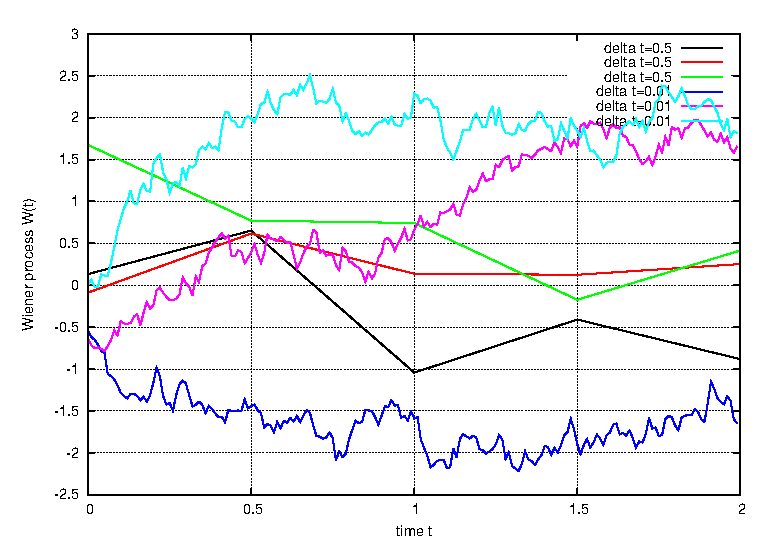
\includegraphics{task10_w}
\caption{3 Wiener processes with parameters $S(0)=10,\mu=0.1,\sigma=0.2,T=2$}
\label{fig:Task10a}
\end{figure}

\begin{figure}[!ht]
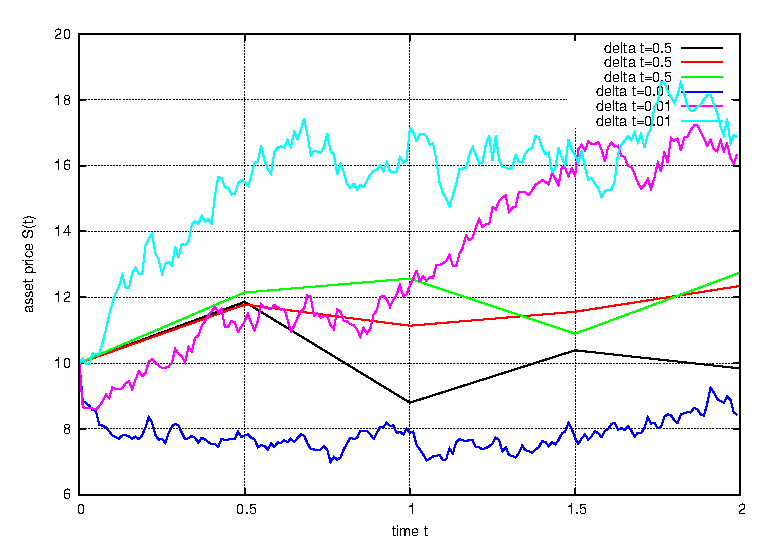
\includegraphics{task10_s}
\caption{corresponding asset prices}
\label{fig:Task10b}
\end{figure}
\clearpage
\end{document}
